\lecture{Computer Structure and Function}{23-01-23}{16:00}{Farzad}{RB LT1}

\textit{We have now finished content relating to Binary and Boolean Algebra. Until Easter (approx 5 weeks) we will be covering the CPU and how it works then until the end of the year, we will look at operating systems and how they work.}

\section{Computers as Complex Systems}
A computer is a complex system. There are two key concepts to understand when referring to how a computer works, computer architecture and computer organisation.
\define{Computer Architecture}{This is the attributes that have a direct impact on the logical execution of a program.}
\define{Computer Organisation}{This referrs to the operational units and their interconnections that realise the architectural operation.}

The difference between these two concepts can be described with the analogy of a car: the architecture of the car will always be the same (cars always need an engine and wheels) however precise organisation (implementation) of the architecture will vary from model to model (some cars may have electric engines and some may have petrol).

This same analogy can be applied to computers: all computers require the same architecture to work however the precise organisation varies from machine to machine (historically vacuum tubes, now we use transistors).

\define{Computer Structure}{The way in which the components are interrelated.}
\define{Computer Function}{The operation of each individual component as part of the structure.}

\subsection{Computer Function}
\marginNote{re-written 2023-04-13}
The computer has four main functions.
\begin{description}
    \item[Data Processing] where the computer manipulates the data for a specific function. There are a wide variety of situations this is important in however there are only a few methods/ types of data processing. 
    \item[Data Storage] where the computer will save data so it can be accessed at a later time/ date. Data can either be stored in the long term (through a low cost Hard Drive/ SSD) or temporarily (through higher cost RAM). 
    \item[Data Movement] where the computer can move data between itself and the outside world. This data will probably interface through \textit{Input/ Output} (I/O) devices. Data movement also concerns peripherals and communication from device to device, this process is known as data communications.
    \item[Control] where the computer must coordinate all the different things which are happening within it. This will encompass data processing, storage and movement. The Control unit manages the computers resources and decides the responses to instructions, including what other components do. 
\end{description}

\subsection{Computer Structure}
Within a computer, there are a number of interrelated components.
\begin{itemize}
    \item Peripherals
    \item Communication Lines
    \item Storage
    \item Processing
\end{itemize}
There are also a number of key components within a computer.
\begin{itemize}
    \item Central Processing Unit (CPU) - controls everything in the computer
    \item Main Memory - stores data
    \item I/O - moves data between the computer and its external environment
    \item System Interconnection (buses) - communicate between the main memory, I/O and CPU
\end{itemize}

\subsubsection{Central Processing Unit}
The CPU has a number of components within it.

\begin{description}
    \item[Arithmetic \& Logic Unit (ALU)] is an adder/ subtracter that perfoms the arithmetic and logical operations (using binary as we learnt in TB1).
    \item[Registers] are very small amounts of extremely fast and very expensive memory which is internal to the CPU. It is used to speed up access to data in turn speeding up CPU performance.
    \item[Internal Bus] is the internal communications line within the CPU.
    \item[Control Unit (CU)] controls the operations of the CPU, which controls the operations of the computer.  
\end{description}

\section{History Of Computers}
\subsection{First Generation}
The first generation of computers used vacuum tubes. The first computer (ENIAC, Electronic Numerical Integrator and Computer) was created during WWII out of need for automating some of the missile launching procedures at the University Of Pennsylvania. It was manually programmed using decimal (not binary) and could do 5000 additions per second. It weighed 30 tones, took up 1500 square feed and contained 18000 vacuum tubes.
\subsection{Next Generation}
The next generation of computers were designed between 1946 and 1952 by Von Neumann. This machine now incorporates the `stored-program concept'. This computer was called an Institute of Advanced Study (IAS) Computer.
\begin{figure}[H]
    \centering
    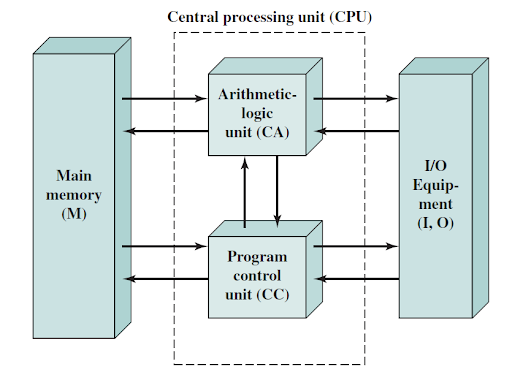
\includegraphics[width=0.8\textwidth]{assets/ias-computer.png}
    \caption{Institute of Advanced Study Computer}
\end{figure}
Memory within the IAS computer had also been re-designed since ENIAC. The memory now had 1000 locations, each 1 word (40 binary bits) long. This could either be used in Number word where the MSB acted as a sign bit or Instruction Mode where there were two instructions per word, each comprised of an 8-bit opcode (what the instruction is) and a 12 bit address (memory location of data to be used in the operation).